\chapter{Constructing A Field Graph} \label{ch:graph_construction}
From the fit Variogram generated as a byproduct of the Kriging method, a metric for the confidence of a prediction can be extrapolated. This metric across the entirety of the target field will be the variable that will be minimized in the objective function of the path planning algorithm introduced.

\section{Field Decomposition Using Voronoi Tessellations}
A \textit{approximate cellular decomposition} will be used to break apart the target field in question. The goal of using this decomposition technique is to cover the entirety of the target field with logical paritions that help achieve the exploration goal \cite{choset:coverage}. The sum of the area of the partitions will be equal to the total area of the target field.

A Voronoi diagram will be generated in order to partition the target field. From a set of sampled locations on a target field, boundaries for natural neighbors are generated from the Voronoi tessellation. The Dirichlet cells, or Voronoi polygons, generated will be referred to as neighbors, where the $i^{th}$ neighbor in the diagram is referred to as $\upsilon_i \in \Upsilon$, the set of all neighbors. The method and implementation in which these cells are generated will not be discussed in this work, but can be referred to in The Handbook of Discrete and Computational Geometry \cite{goodman:voronoi}. The points used to generate the neighborhood will be a handful of the coordinates associated with the highest variances of prediction on the target field. The objective of the path planning algorithm introduced will be to minimize the total uncertainty of the predictions on the entirety of a target field. If a variance drop occurs in a neighborhood when the cell is visited and observed, the variance associated with a field as a whole will be minimized.

A graph representing the confidence of prediction for each neighborhood can be generated. The confidence of a neighborhood, inversely proportional to its uncertainty. Neighbors adjacent in the tessellated field are placed in the graph representation as adjacent vertices. For two given vertices in the graph, $\upsilon_i$ and $\upsilon_j$, the corresponding edge weight, $w_{ij}=2_{ji}$ is the sum of the proportional confidences of the two associated neighborhoods, where the uncertainty of neighborhood will be the maximum variance in the area.

\section{Relationship Between Vornoi Cells and The Kriging Proximity Vector}
idk

\begin{equation}
    w_{ij} = w_{ji} = \frac{1}{var\{\upsilon_i\}} + \frac{1}{var\{\upsilon_j\}}
\end{equation}

\begin{figure}[thpb]
\centering
    \begin{subfigure}[b]{\textwidth}
        \centering
        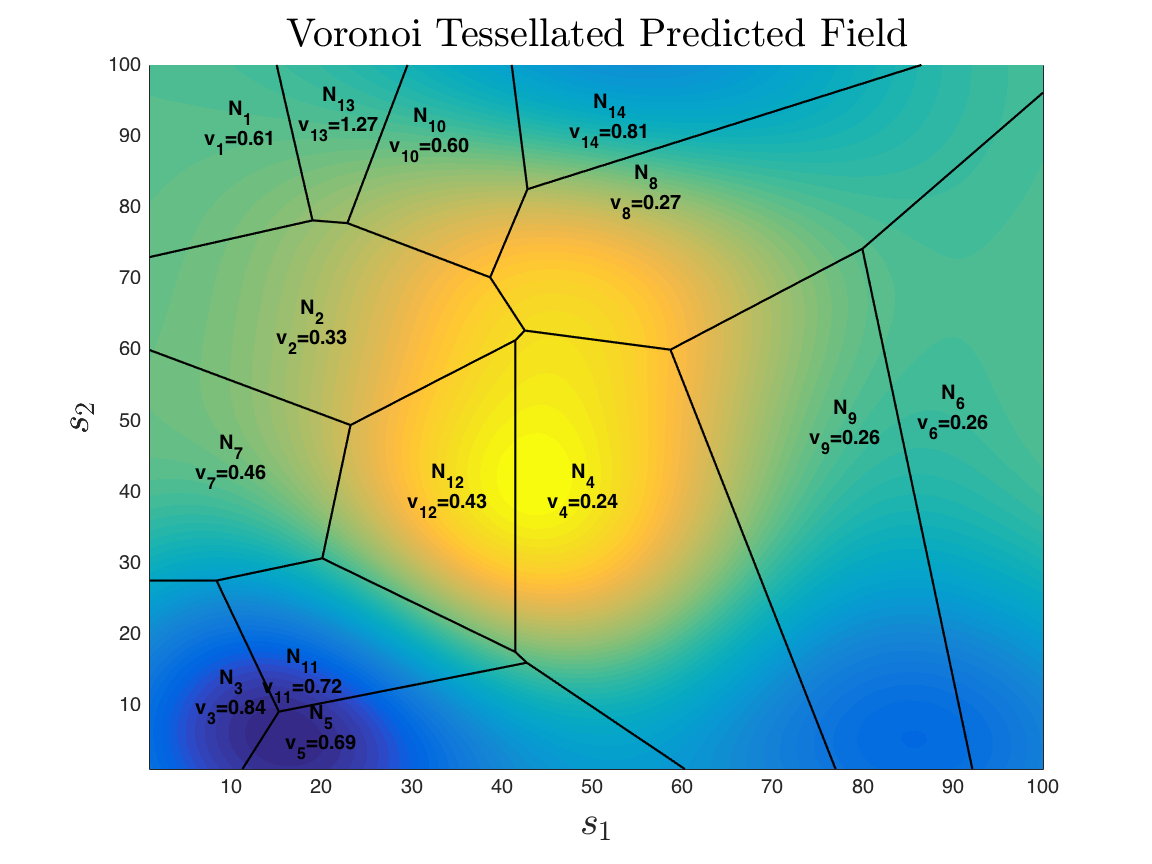
\includegraphics[width=0.8\textwidth]{./figures/natural_neighborhood_selection.png}
        \captionsetup{skip=0.0\baselineskip,size=footnotesize}
        \caption{Voronoi tessellations of the predicted field in Figure \ref{fig:krig_field}. In this figure, a cell is associated with each observation location.}
        \label{fig:nat_neigh}
    \end{subfigure}
    \\
    \begin{subfigure}[b]{\textwidth}
        % \includegraphics[width=0.7\textwidth]{./figures/undir_graph_save.png}

        %https://tex.stackexchange.com/questions/270543/draw-a-graph-in-latex-with-tikz
        \centering
        \begin{tikzpicture}
        \begin{scope}[every node/.style={circle,thick,draw}]
            \node (N4) at (0.2,3) {$N_4$};
            \node (N2) at (1.6,.6) {$N_2$};
            \node (N7) at (4.5,.4) {$N_{7}$};
            \node (N12) at (2.7,3) {$N_{12}$};
            
        \end{scope}

        \begin{scope}[>={Stealth[black]},
                      every node/.style={fill=white,circle},
                      every edge/.style={draw=red,very thick}]

            \draw (N7) -- (4.6,1.8) [dashed];
            \draw (N7) -- (5.0,1.6) [dashed];

            \draw (N2) -- (0.4,1.5) [dashed];
            \draw (N2) -- (0.4,1.1) [dashed];
            \draw (N2) -- (0.0,0.9) [dashed];
            \draw (N2) -- (2.6,1.3) [dashed];

            \draw (N4) -- (1.0,2.6) [dashed];
            \draw (N4) -- (0.9,2.4) [dashed];
            \draw (N4) -- (0.4,1.8) [dashed];
            \draw (N4) -- (0,2.0) [dashed];

            \draw (N12) -- (3.9,2.7) [dashed];
            % edge[bend right=90] node
            \path [-] (N4) edge node {$w_{4,2}$} (N2);
            \path [-] (N4) edge node {$w_{4,12}$} (N12);
            \path [-] (N12) edge node {$w_{12,2}$} (N2);
            \path [-] (N12) edge node {$w_{12,7}$} (N7);
            \path [-] (N2) edge node {$w_{2,7}$} (N7);
            

        \end{scope}
        \end{tikzpicture}

        \captionsetup{skip=0.5\baselineskip,size=footnotesize}
        \caption{A subset of the weighted graph representing the adjacencies of the neighbors in Figure \ref{fig:nat_neigh}}
        \label{fig:neigh_graph}
  \end{subfigure}
  \captionsetup{skip=0.5\baselineskip,size=small}
  \caption{The predicted field is tessellated based on the measured point locations in \ref{fig:nat_neigh}. An undirected graph is constructed from the tessellations in \ref{fig:neigh_graph}. The label in each neighborhood identifies the neighborhood name, $\upsilon_i$, and the associated confidence of prediction, $\nu_i$, for that neighborhood.}
\end{figure}

Typically, only $k$ neighbors will be generated from a set of the $k$ highest variances in the variance of the target field prediction. This is done in an effort to reduce the computational intensity of tessellating a field and constructing/traversing a graph as the number of total observations increases.